% This line sets the project root file.
% !TEX root = Notes_Gauging_Defects.tex
% !TEX spellcheck = en_US

\subsection{Example: Spin chain}
\label{subsec:VecZ2}

We consider a one-dimensional spin chain of $N$ particles, where each particle can be in the spin-up state or in the spin-down state, i.e., a chain
	\begin{figure}[H]
		\centering
		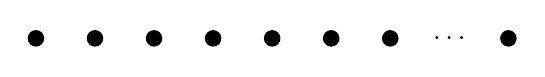
\begin{tikzpicture}[scale=1.5]
			\fill[black] (0,0) circle (0.07cm);
			\fill[black] (0.5,0) circle (0.07cm);
			\fill[black] (1,0) circle (0.07cm);
			\fill[black] (1.5,0) circle (0.07cm);
			\fill[black] (2,0) circle (0.07cm);
			\fill[black] (2.5,0) circle (0.07cm);
			\fill[black] (3,0) circle (0.07cm);
			\fill[black] (4,0) circle (0.07cm);
			\node at (3.5,0) {$\dots$};
		\end{tikzpicture}
	\end{figure}
\noindent
whose Hilbert space is 
	\begin{equation}
		\mathcal{H}_0=\bigotimes_{i=1}^N \mathbb{C}^2.
	\end{equation}
We now introduce defects, which means that one of the spins, say the spin at site $j$, is replaced by a different kind of spin, e.g., no spin (indicated in red): 
	\begin{figure}[H]
		\centering
		\begin{tikzpicture}[scale=1.5]
			\fill[black] (0,0) circle (0.07cm);
			\fill[black] (0.5,0) circle (0.07cm);
			\fill[black] (1,0) circle (0.07cm);
			\fill[black] (1.5,0) circle (0.07cm);
			\fill[bwred] (2,0) circle (0.07cm);
			\fill[black] (2.5,0) circle (0.07cm);
			\fill[black] (3,0) circle (0.07cm);
			\fill[black] (4,0) circle (0.07cm);
			\node at (3.5,0) {$\dots$};
		\end{tikzpicture}
	\end{figure}
\noindent
This corresponds to replacing the Hilbert space $\mathbb{C}^2$ at site $j$ with $\mathbb{C}$, which results in the overall Hilbert space
	\begin{equation}
		\mathcal{H}_1^{(j)}=\left(\bigotimes_{i=1}^{j-1}\mathbb{C}^2\right)\otimes\mathbb{C}\otimes\left(\bigotimes_{i=j+1}^N\mathbb{C}^2\right).
	\end{equation}
The subscript here denotes the number of defects in the chain and the superscript indicates at which site the defect appears. If we want to consider both possibilities, having no defect and having a defect at site $j$, we use the Hilbert space
	\begin{equation}
		\mathcal{H}=\mathcal{H}_0\oplus\mathcal{H}_1^{(j)}.
	\end{equation}
We can also allow the defect to move, which means we still restrict the setting to only one defect in total, but it can happen at any site. Hence, the overall Hilbert space becomes
	\begin{equation}
		\mathcal{H}=\mathcal{H}_0\oplus\left(\bigoplus_{j=1}^N\mathcal{H}_1^{(j)}\right).
	\end{equation}
This construction can be generalized to an arbitrary number of defects: The Hilbert space for having defects two defects in the chain, say at sites $j$ and $k$, is 
	\begin{equation}
		\mathcal{H}_2^{(j,k)}=\left(\bigotimes_{i=1}^{j-1}\mathbb{C}^2\right)\otimes\mathbb{C}\otimes\left(\bigotimes_{i=j+1}^{k-1}\mathbb{C}^2\right)\otimes\mathbb{C}\otimes\left(\bigotimes_{i=k+1}^{N}\mathbb{C}^2\right).
	\end{equation}
Again, if we allow these defects to move and also include the possibilities of having only one defect and no defect at all, the overall Hilbert space is
	\begin{equation}
		\mathcal{H}=\mathcal{H}_0\oplus\left(\bigoplus_{j=1}^N\mathcal{H}_1^{(j)}\right)\oplus\left(\bigoplus_{j=1}^N\bigoplus_{k\neq j}\mathcal{H}_2^{(j,k)}\right).
	\end{equation}
We can continue this construction until we have a defect at every site of the chain, i.e.
	\begin{equation}
		\mathcal{H}_N=\bigotimes_{i=1}^N\mathbb{C},
	\end{equation}
and the overall Hilbert space is then
	\begin{equation}
		\mathcal{H}=\bigoplus_{n\in\#\mathrm{defects}}\mathcal{H}_n,
	\end{equation}
where $\mathcal{H}_n$ is the direct sum of all possible Hilbert spaces with $n$ defects, as constructed above. Since this is now a very complicated Hilbert space, we can also think about it in a different and simpler way: at each site, the particle can be in one of three states: spin up, spin down, or no spin. Hence, we have effectively a three-level system at each site of the chain, and therefore the overall Hilbert space can be written as
	\begin{equation}
		\mathcal{H}\cong\bigotimes_{j=1}^N\left(\mathbb{C}\oplus\mathbb{C}^2\right).
	\end{equation}

We study a concrete example in detail in Sec.~\ref{Ising}, namely a particle chain in the sense of the golden chain presented in \cite{Feiguin2007}, which is based on a fusion category with $\Vec(\Z/2\Z)$ fusion rules with pairwise interaction. Since the discussion of this example requires some background on fusion categories and bimodules as well as annular categories, we present the mathematical preliminaries in the next section before explicitly constructing the defects afterwards.

